
% ---------------------------------------------------------------------------
% Lauter et al. (2005) Example 3 -- exact analytic solution (unsteady solid-body
% rotation with a precessing rotation axis). Requires \usepackage{amsmath}.
% ---------------------------------------------------------------------------
The L\"auter et al.\ (2005) Example~3 test case is an unsteady exact solution of the
rotating shallow water equations: solid-body rotation about an axis that precesses
around the polar axis at the planetary rotation rate~$\Omega$. With sphere
radius~$a$, the time-dependent rotation axis is
%
\begin{equation}
  \mathbf{c}(t) = -\sin\alpha\,\cos(\Omega t)\,\mathbf{e}_1
                  + \sin\alpha\,\sin(\Omega t)\,\mathbf{e}_2
                  + \cos\alpha\,\mathbf{e}_3 ,
  \label{eq:lauter-axis}
\end{equation}
%
and the exact velocity, layer depth and (centrifugal) orography fields are
%
\begin{align}
  \mathbf{u}(\mathbf{x},t) &= \frac{u_0}{a}\,\mathbf{c}(t)\times\mathbf{x}, \label{eq:lauter-u}\\
  g\,D(\mathbf{x},t)       &= k_1 - k_2
       - \tfrac12\!\left(u_0\,\mathbf{c}(t)\cdot\hat{\mathbf{x}} + \Omega z\right)^{2},
       \label{eq:lauter-D}\\
  g\,b(\mathbf{x})         &= \tfrac12\,\Omega^{2} z^{2} + k_2 ,
       \label{eq:lauter-b}
\end{align}
%
where $\mathbf{x}=(x,y,z)$ are Cartesian coordinates, $\hat{\mathbf{x}}=\mathbf{x}/a$
is the outward unit normal and $z=\mathbf{x}\cdot\mathbf{e}_3$. The parameters are
$a = 6{,}371{,}220~\mathrm{m}$, $\alpha = \pi/4$,
$u_0 = 2\pi a/(12~\mathrm{days}) \approx 38.6~\mathrm{m\,s^{-1}}$,
$\Omega = 7.292\times10^{-5}~\mathrm{s^{-1}}$, $g = 9.8~\mathrm{m\,s^{-2}}$,
$k_1 = 133{,}681~\mathrm{m^2\,s^{-2}}$ and $k_2 = 0$, integrated to
$t = 43{,}200~\mathrm{s}$ ($12~\mathrm{h}$).



% Spatial convergence table — Lauter et al. (2005) Example 3, deterministic (--pure).
% cPG P1 in time, BDM2/DG1 in space, coords_degree=2 (quadratic sphere geometry).
% nsteps=2000 (dt=21.6 s, tmax=43200 s); errors are relative L2 vs the exact solution.
% Requires \usepackage{booktabs}.
\begin{table}[htbp]
  \centering
  \begin{tabular}{c c c c c c}
    \toprule
    ref & $h$ (km) & $\|u-u_{\mathrm{ex}}\|/\|u_{\mathrm{ex}}\|$ & rate$_u$
        & $\|D-D_{\mathrm{ex}}\|/\|D_{\mathrm{ex}}\|$ & rate$_D$ \\
    \midrule
    2 & 1785.5 & $1.60\times10^{-2}$ & --   & $4.11\times10^{-3}$ & --   \\
    3 &  892.8 & $2.38\times10^{-3}$ & 2.75 & $1.04\times10^{-3}$ & 1.99 \\
    4 &  446.4 & $4.93\times10^{-4}$ & 2.27 & $2.60\times10^{-4}$ & 2.00 \\
    5 &  223.2 & $1.14\times10^{-4}$ & 2.11 & $6.51\times10^{-5}$ & 2.00 \\
    \bottomrule
  \end{tabular}
  \caption{Spatial convergence for the Läuter et al.\ (2005) Example~3 test case
    (deterministic) using the cPG ($P_1$) time integrator with $\Delta t = 21.6$\,s
    (\texttt{nsteps}$=2000$) at $t = 43200$\,s. Relative $L^2$ errors are measured
    against the exact solution on an icosahedral sphere mesh with quadratic
    coordinate geometry (\texttt{coords\_degree}$=2$), BDM$_2$/DG$_1$ spaces.
    Both the velocity $u$ and depth $D$ converge at second order.}
  \label{tab:lauter-spatial-coords2}
\end{table}

% ---------------------------------------------------------------------------
% Diagnostic figures. Requires \usepackage{graphicx}.
% Upload lauter_div_norms.png and lauter_energy_errors.png to the Overleaf project.
% ---------------------------------------------------------------------------
\begin{figure}[htbp]
  \centering
  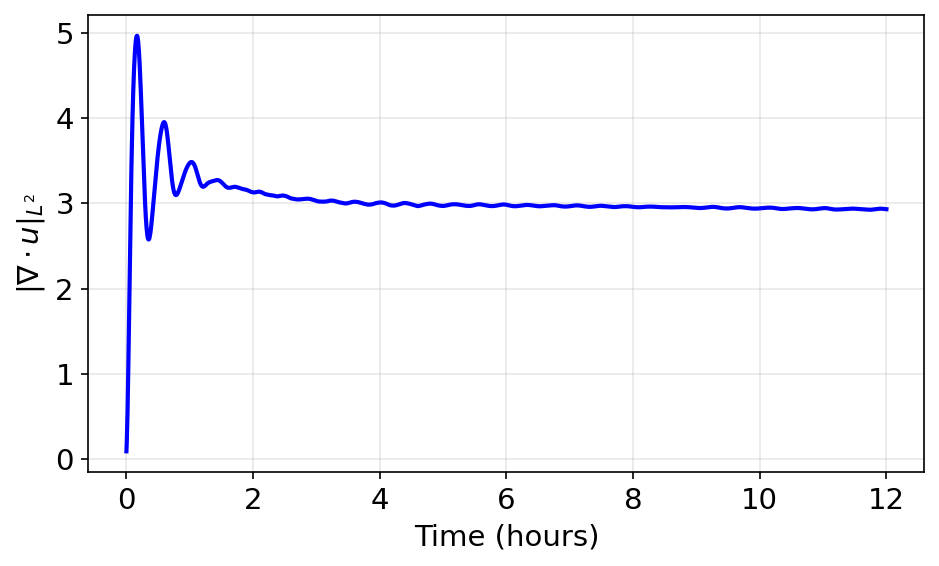
\includegraphics[width=0.8\textwidth]{lauter_div_norms.png}
  \caption{Time evolution of the velocity divergence $\|\nabla\cdot u\|_{L^2}$ for the
    Läuter et al.\ (2005) Example~3 test case (deterministic), cPG ($P_1$) on a fixed
    mesh (refinement level~4, \texttt{coords\_degree}$=2$, $\Delta t = 42.2$\,s).
    The initial gravity-wave adjustment damps to a steady value within a few hours.}
  \label{fig:lauter-div}
\end{figure}

\begin{figure}[htbp]
  \centering
  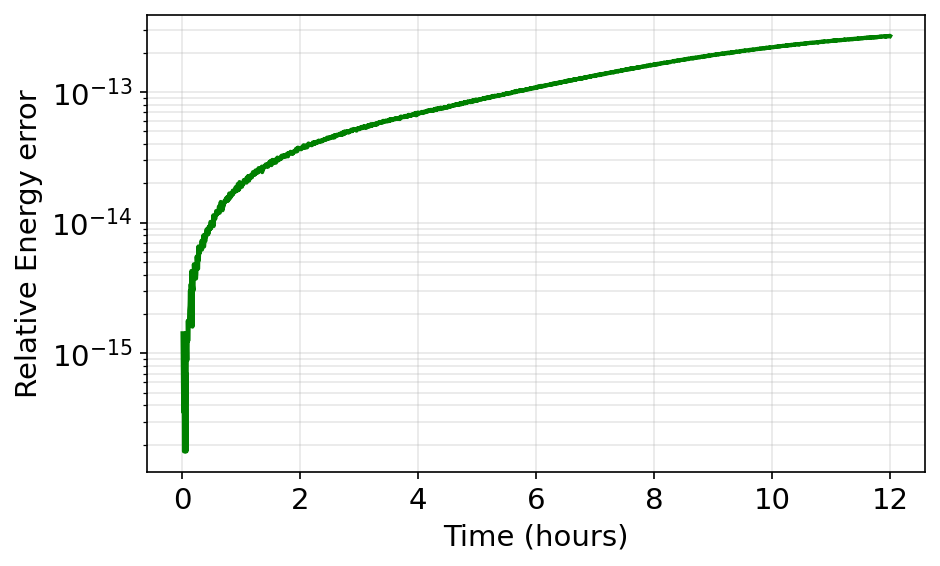
\includegraphics[width=0.8\textwidth]{lauter_energy_errors.png}
  \caption{Relative energy drift $|(E-E_0)/E_0|$ for the Läuter et al.\ (2005)
    Example~3 test case (deterministic), cPG ($P_1$) on a fixed mesh (refinement
    level~4, \texttt{coords\_degree}$=2$, $\Delta t = 42.2$\,s). The energy is
    conserved to solver/round-off precision ($\sim 10^{-13}$) throughout the run,
    confirming the energy-conserving property of the fully discrete scheme.}
  \label{fig:lauter-energy}
\end{figure}

